Der Link Layer nutzt ein gemeinsames Paketformat für das Übertragen von Advertising-Paketen und Nutzdaten-Pakten, das in Abb. \ref{fig: ll paket struktur} dargestellt ist.\\

\begin{figure}[H]
    \centering
    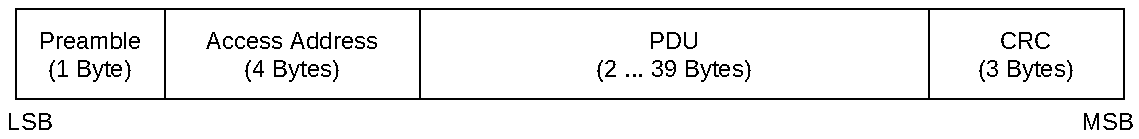
\includegraphics[width=0.9\textwidth]{graphics/link_layer_packetformat.pdf}
    \caption[Paketstruktur des Link Layers]{Paketstruktur des Link Layers; in Anlehnung an \cite{BtSpec4.0_fig_2200}}
    \label{fig: ll paket struktur}
\end{figure}
% QUELLE Spec 4.0 S. 2200 - 2201

Die Preamble hat eine Größe von acht Bit und wird genutzt, um auf Empfängerseite die Frequenz zu synchronisieren, die Zeiteinteilung der Symbole zu schätzen und um die Automatic Gain Control zu trainieren. Die Preamble beträgt immer 0b01010101, falls das Bit mit dem niedrigsten Stellenwert (LSB für Least Significant Bit) der Access Address 1 ist. Anderenfalls beträgt die Preamble 0b10101010. \cite{BtSpec4.0_2200-2201}
\\\\
Die Access Address hat eine Größe von 32 Bit und identifziert eine Verbindung über den Link Layer bzw. dient dazu, Pakete mittels des festgelegten Wertes 0x8E89BED6 als Advertisement-Pakete zu identifzieren. Bevor ein Initiator eine Verbindung zu einem Advertiser aufbaut, erstellt er eine zufällige Access Address, die neben weiteren Bedingungen nicht der des Advertisement"=Pakets gleichen oder sich nur um ein Bit von ihr unterscheiden darf. Diese Access Address sendet er dann innerhalb der Verbindungsanfrage an den Advertiser. \cite{BtSpec4.0_2200-2201}
\\\\
Das letzte Feld des Link-Layer-Pakets ist der 24 Bit lange Cyclic Redundancy Check (CRC), der über das PDU-Feld berechnet wird. Im Fall, dass auf Ebene des Link Layers die PDU verschlüsselt wird, generiert man den CRC erst nach der Verschlüsselung. Unabhängig davon, ob die Verschlüsselung aktiv ist, wird anschließend ein Whitening \cite{BtSpec4.0_2217-2218} durchgeführt, um Sequenzen vieler gleichbleibender Bits (bspw. 0b00000000) zu verhindern. \cite{BtSpec4.0_2200-2201}
% QUELLE Spec 4.0 S. 2217-2218
\\\\
Die Protocol Data Unit (PDU) unterteilt sich in die Advertising Channel PDU und Data Channel PDU.

\subparagraph{Advertising Channel PDU} \mbox{} \vspace{0.2cm} \\
Wie in Abb. \ref{fig: ll adv channel pdu} gezeigt wird, besteht die Advertising Channel PDU aus einem 16 Bit langen Header und einem Payload variabler Länge. RFU steht dabei für Reserved for Future Use.

\begin{figure}[H]
    \centering
    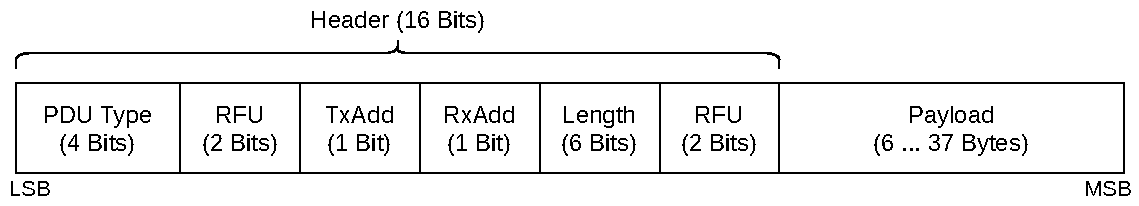
\includegraphics[width=0.9\textwidth]{graphics/link_layer_packetformat_pdu_adv.pdf}
    \caption[Link Layer Advertising Channel PDU]{Link Layer Advertising Channel PDU; in Anlehnung an \cite{BtSpec_fig_2201} und \cite{BtSpec_fig_2202}}
    \label{fig: ll adv channel pdu}
\end{figure}
% QUELLE advertising channel pdu format S. 2201 f.

Dabei beinhaltet der Header unter anderem ein 4 Bit langes Feld für den PDU Type (bspw. Connectable Undirected Advertising Event oder Scan Request) und zwei Flags TxAdd und RxAdd für zusätzliche Informationen bezüglich des PDU Type. Die Bedeutungen von TxAdd und RxAdd hängen vom PDU Type ab. Die Menge aller PDU Types lässt sich folgendermaßen untergliedern:
\begin{itemize}
    \item Advertising PDU
    \item Scanning PDU
    \item Initiating PDU
\end{itemize}
Bei allen bilden die ersten 6 Bytes des Payload die Adresse des Senders (Advertiser, Scanner oder Initiator). Hier sagt TxAdd bei jedem PDU Type aus, ob die angegebene Adresse des Senders öffentlich (TxAdd = 0) oder zufällig generiert (TxAdd = 1) ist. Diese Funktion wird Privacy Feature gennant und ist in Sektion \ref{sec: gap sicherheit} genauer beschrieben. RxAdd dagegen ist nur bei PDU Types von Bedeutung, die in ihrem Payload eine zweite Adresse enthalten, nämlich die des Empfängers. Analog zu TxAdd sagt RxAdd aus, ob die Adresse des Empfängers öffentlich (RxAdd = 0) oder zufällig (RxAdd = 1) ist.

Ein weiteres Feld im Header der Advertising Channel PDU ist das 6 Bit lange Feld für die Länge des Payloads in Bytes, dessen Wert eine Spanne von 6 bis 37 Byte abdeckt. \cite{BtSpec4.0_2201-2208}
\\\\
\subparagraph{Data Channel PDU} \mbox{} \vspace{0.2cm} \\
Die Data Channel PDU nutzt entsprechend der Abb. \ref{fig: ll data channel pdu} einen 16 Bit langen Header, einen Payload variabler Länge und optional einen 32 Bit langen Message Integry Check (MIC), der die Integrität des Payload sicherstellt. Das MIC-Feld entfällt bei einer unverschlüsselten Link-Layer-Verbindung und bei einer Data Channel PDU, deren Payload leer ist.

\begin{figure}[H]
    \centering
    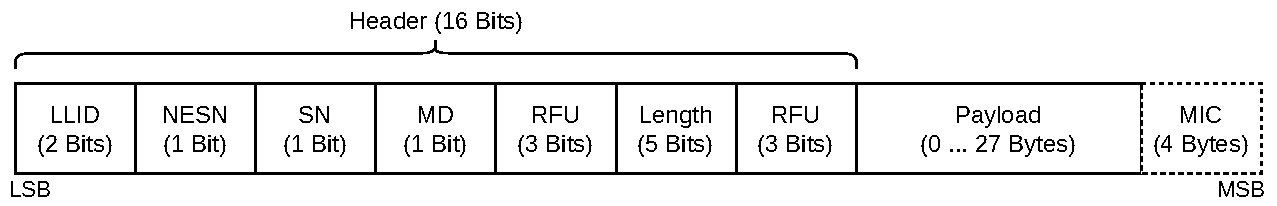
\includegraphics[width=1\textwidth]{graphics/link_layer_packetformat_pdu_data.pdf}
    \caption[Link Layer Data Channel PDU]{Link Layer Data Channel PDU; in Anlehnung an \cite{BtSpec_fig_2208a} und \cite{BtSpec_fig_2208b}}
    \label{fig: ll data channel pdu}
\end{figure}

Das erste Feld des Headers ist der zwei Bit lange Link Layer Identifier (LLID), der mit 0b01 sowie 0b10 aussagt, dass es sich um eine LL Data PDU handelt und mit 0b11, dass es sich um eine LL Control PDU handelt. Der Wert 0b00 ist reserviert. Die LL Control PDU dient dazu, die LL-Verbindung zu steuern. Dazu gehören unter anderem Anfragen zum Ändern der Verbindungsparameter (z.B. Window Size oder Timeout), zum Ändern der Channel Map oder zum Verschlüsseln.

Auf die LLID folgt das Feld der Next Expected Sequence Number (NESN) und das Feld der Sequence Number (SN) mit jeweils einem Bit Länge, die innerhalb Sektion \ref{sec: le ll transport} näher erläutert werden.

Unter anderem beinhaltet der Header ein fünf Bit langes Feld für die Länge des Payload in Byte und ggf. einschließlich der Länge des MIC. Der maximale Wert der Länge beträgt 31 Bytes, wobei sich der Payload in jedem Fall auf eine maximale Länge von 27 Bytes bemisst. \cite{BtSpec4.0_2208-2209}

In der Bluetooth-Version 4.2 ist das Feld der Länge auf acht Bit erweitert, wodurch der Payload eine maximale Größe von 251 Bytes annehmen kann. \cite{BtSpec4.2_2589-2590}